%
%  untitled
%
%  Created by Joan T. Matamalas Llodrà on 2011-04-19.
%  Copyright (c) 2011 __MyCompanyName__. All rights reserved.
%
\documentclass[12pt, a4paper]{article}

% Use utf-8 encoding for foreign characters
\usepackage[utf8]{inputenc}
\usepackage{eurosym}

% Setup for fullpage use
\usepackage{fullpage}

% Uncomment some of the following if you use the features
%
% Running Headers and footers
%\usepackage{fancyhdr}

% Multipart figures
\usepackage{subfigure}

% More symbols
%\usepackage{amsmath}
%\usepackage{amssymb}
%\usepackage{latexsym}

% Surround parts of graphics with box
\usepackage{boxedminipage}

% Package for including code in the document
\usepackage{listings}

% Multirow tables
\usepackage{multirow} 

% Cell color
\usepackage[table]{xcolor}

% If you want to generate a toc for each chapter (use with book)
\usepackage{minitoc}

% This is now the recommended way for checking for PDFLaTeX:
\usepackage{ifpdf}

%\newif\ifpdf
%\ifx\pdfoutput\undefined
%\pdffalse % we are not running PDFLaTeX
%\else
%\pdfoutput=1 % we are running PDFLaTeX
%\pdftrue
%\fi

\ifpdf
\usepackage[pdftex]{graphicx}
\else
\usepackage{graphicx}
\fi
\title{Introduction to Machine Learning\\Work 1\\Clustering and factor analysis exercise}
\author{Marc Oliu Simón\\Joan T. Matamalas Llodrà}

\date{\today}

\begin{document}

\ifpdf
\DeclareGraphicsExtensions{.pdf, .jpg, .png, .BMP}
\else
\DeclareGraphicsExtensions{.eps, .jpg}
\fi

\maketitle

\section{Parsing the files} % (fold)
\label{sec:parsing_the_files}
\paragraph{}The first step in the development of both K-Means and PCA algorithms has been the development of a parsing function for the ARFF files. For this purpose, the documents have been read line by line, and the comment lines, empty lines and types definition lines have been discarded.\\

The signature for the function is the following one:
\[
	function[matrix] = parser\_ariff(path)
\]
\paragraph{}As it can be seen, the input value is the path of the data set to load, while the output value is an array of integers representing the matrix parsed from the input file.\\

The lines containing the matrix data have been parsed by converting the comma-separated rows (which represent individuals of the population) into their fields, and the column representing the classification of those individuals have been discarded. That is so because the goal of the practice is to implement an unsupervised classifier, and thus there is no need to maintain the classifier for each element.\\

For the fields containing unknown values, a NaN (Not a Number) value has been assigned in order to transform the rest of the fields from strings to numeric values.
% section parsing_the_files (end)

\section{Standardizing the data and assigning missing values} % (fold)
\label{sec:standardizing_the_data_and_assigning_missing_values}
\paragraph{}Once the matrix is obtained, the data is standardized to give an equal importance to all the fields of the data, and in the process the value for the outliers is assigned.\\

A standardization process has been chosen over normalization because of the continuous nature of the variables. Since the variables of the data set represent a continuous value over the feature, and since the features follow a normal distribution, it's better to standardize to avoid features containing elements at various standard deviations from the mean from gaining importance over the features not containing them.\\

For example, if a feature had an individual past the second standard deviation (P $<$ 0.95) this feature data would be more compressed if normalized than another without any individual past the second standard deviation, since this individual would have a value of 0 or 1 for this feature.\\

On the other hand, when standardizing, 67\% of the population will fall within one standard deviation, independently of the existence of outliers or low probability individuals that could fall past the second standard deviation.\\

The function developed to perform the standardization and assignment of missing values has the following signature:
\[
	function[matrixZ] = standarizer(matrix)
\]

\paragraph{}The process followed to standardize the data is the following one for each feature:
\begin{enumerate}
	\item Calculate the mean of the feature ignoring the unknown values (NaNs)
	\item Assign the obtained mean to the unknown values
	\item Standardize the feature
\end{enumerate}
\paragraph{}This process is done simultaneously for all features of the data set by working with all of the columns (features) of the matrix at the same time.
% section standardizing_the_data_and_assigning_missing_values (end)

\section{Implementation of the K-Means} % (fold)
\label{sec:implementation_of_the_k_means}

\subsection{The K-Means Function} % (fold)
\label{sub:the_k_means_function}
\paragraph{}The K-Means algorithm has been implemented inside a function named k\_means, which has the following signature:
\[
function [ best\_output, best\_centroids, best\_inertia ] = k\_means( dataMatrix, k, seed, repetitions )
\]
\paragraph{}As it can be seen, the function accepts three input parameters, and gives three parameters as output. The input parameters represent the following:
\begin{itemize}
	\item \textbf{dataMatrix:} This parameter is the matrix over which the k-means algorithm will perform the clustering. Each row of the matrix is an individual of the population and each column one of the features.
	\item \textbf{k:} Is the number of clusters the data will be classified in.
	\item \textbf{seed:} It's an integer number used as seed for a random number generator. The method to select the initial seeds of the K-Means algorithm consists on assigning each individual to a cluster and then calculating the centroids of each cluster. \emph{Default 1}
	\item \textbf{repetitions:} Number of repetitions of the algorithm, returns the best clusters so far. \emph{Default 1}
\end{itemize}
\paragraph{}The three output parameters of this function are the following ones:
\begin{itemize}
	\item \textbf{best\_output:} Vector with the best cluster for each individual obtained after n repetitions.
	\item \textbf{best\_centroids:} Centroids of the clusters (1 row per cluster)
	\item \textbf{best\_inertia:} Vector with the inertia of each cluster
\end{itemize}
\paragraph{}Our K-Means algorithm implementation starts out by assigning each individual to one of the K clusters randomly, and then calculating it's centroids. This way, the initial seeds are obtained for the algorithm to run. Then it clusters the individuals to the centroids by using the euclidean distance between each individual and each centroid, assigning the individual to the nearest centroid.\\

This process is repeated iteratively, Recalculating the centroids for the new clusters and then creating the clusters again using the newly calculated centroids to assign the individuals to each cluster. The process stops when there is convergence, that is, the centroids don't change anymore and each individual is re-assigned to the same cluster to which it was assigned the previous iteration.
% subsection the_k_means_function (end)

\subsection{Generating and selecting the clusters} % (fold)
\label{sub:generating_and_selecting_the_clusters}
\paragraph{}To generate the clusters for the K-Means classifier, an iterative process has been implemented, in which the data is clustered for values of K ranging from 2 to 5, and for each value of K different seeds are tried.\\

Since the seed in our implementation is an integer value that is used as the seed of a random number generator which in turn creates an initial random clustering of the data, a range of numbers from 1 to 25  is tried to generate the initial seeds for the clusters.\\

From the different seeds used, the best clustering is selected by using the clusters internal inertia as evaluation method. For the clusters with the same value of K, the one that has the lowest inner cluster inertia are considered the best, since the distance between the cluster members and their centroids is minimized, meaning the clusters are more compact.\\

Unfortunately, this same procedure can't be used to evaluate which is the best value of K. This is because a higher value of K always minimizes the inner cluster inertia, and the best value would turn out to be a K value equal to the number of individuals in the data set (cluster inertia = 0). For that reason, the K-Means algorithm is run for the different K values, and a reduced dimensionality 3D plot is shown for each value of K, by applying Multi Dimensional Scaling (MDS), allowing for a manual selection of the best K value.
% subsection generating_and_selecting_the_clusters (end)
% section implementation_of_the_k_means (end)

\section{Implementation of the PCA} % (fold)
\label{sec:implementation_of_the_pca}
\paragraph{}The PCA is implemented in the function \emph{pca}. The signature of that function is:
\[
	function [ outData, transformedData, eVectors, eValues, informativeFeatures] =
\]
\[
	=pca( dataMatrix, eValueThreshold)
\]
\paragraph{}The inputs parameters are:
\begin{itemize}
	\item \textbf{dataMatrix:} This parameter is the matrix over which the k-means algorithm will perform the clustering. Each row of the matrix is an individual of the population and each column one of the features.
	\item \textbf{eValueThreshold:} The minimum value of an eigenvalue to accept the associate eigenvector as featured vector.
\end{itemize}
\paragraph{}As output the function provides:
\begin{itemize}
	\item \textbf{outData:} The data in the original coordinates with the reduction of dimensions applied.
	\item \textbf{trasnfomedData:} The transformed data with dimensions reduced
	\item \textbf{eVectors:} eigenVectors of the data
	\item \textbf{eValues:} eValues of the data
	\item \textbf{informativeFeatures:} the index of the most informative attributes
\end{itemize}

\paragraph{}The principal component analysis (PCA) is a procedure used to reduce the dimensionality of the original data. The steps in what the algorithm is decomposed are:
\begin{enumerate}
	\item \textbf{Subtract the mean from data: }This step was omitted. The algorithm works with standardized data, so we've already subtracted the mean in the standardization step.
	\item \textbf{Calculate the convariance matrix:} This is an important step that gives us information about the variance of the several attributes. We have used the \emph{cov} function to obtain this details.
	\item \textbf{Calculate the eigenvectors and eigenvalues of covariance matrix:} Matlab has a function that does that task (\emph{eig}). The function returns a matrix with the eigenvectors and other with the eigenvalues on the diagonal. Both are ascendent ordered so we need to revert that in order to keep them in descendent order. The eigenvalues are put in a column with the command \emph{diag} in order to be more useful.
	\item \textbf{Choose components and construct a new featured vectors set:} We have to choose the most informative attributes to represent the data. We have created a matrix containing the vectors that have eigenvalues above a determined threshold, by default 1.
	\item \textbf{Transform the original data based on the set of featured vectors:} Now, with the featured eigenvectors in our hands, we can proceed to transform our original data. To do that, we multiplay the transposed version of the featured vectors matrix by the transposed data matrix. That result will have n number of dimensions, where n is the number of eigenvectors selected.
	\item \textbf{Reconstruct the old data back:} If we wanna reconstruct the data in our originals coordinates we would multiply the matrix of featured vectors by the matrix obtained in the previous step.
\end{enumerate}
\paragraph{}Additionally to this steps, we need to know which attributes have more information. To do that, we choose from the absolute values of each featured vector the maximum value, the index of this maximum is the index the attribute that we need.
% section implementation_of_the_pca (end)

\section{Analysis of the data sets} % (fold)
\label{sec:analysis_of_the_data_sets}

\subsection{Data set: Pima Indians Diabetes Database} % (fold)
\label{sub:data_set_pima_indians_diabetes_database}
\textbf{File:} pima\_diabetes.arff\\

This dataset corresponds to a study of the diabetes disease over a population of Pima indians. For the analysis, a group of 8  variables were taken into account, which are:

\begin{enumerate}
	\item Number of times pregnant
	\item Plasma glucose concentration a 2 hours in an oral glucose tolerance test
	\item Diastolic blood pressure (mm Hg)
	\item Triceps skin fold thickness (mm)
	\item 2-Hour serum insulin (mu U/ml)
	\item Body mass index (weight in kg/(height in m)$^2$)
	\item Diabetes pedigree function
	\item Age (years)
\end{enumerate}

\paragraph{}Each of the individuals has been classified as having diabetes or not, but for the purpose of this work, the classification isn't required. The first step in the analysis of the data will be to try a classification of the individuals by using the K-Means classifier with different values of K. The figure~\ref{fig:diabetes_1} show the result of this classification.
\begin{figure}[ht!]
	\centering
	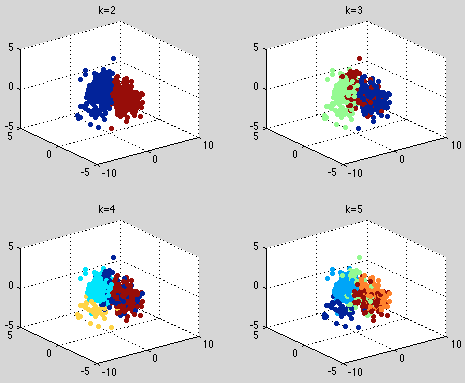
\includegraphics[width=0.55\textwidth]{img/Diabetes_1}
	\caption{k-means clustering for diabetes data without use PCA}
	\label{fig:diabetes_1}
\end{figure}
\paragraph{}For each consecutive K value, the inertia of the clusters is further reduced, as expected. Since the above representation is a 3D representation of an 8-dimensional space, it's hard to tell which K value gives a better separation between clusters, although it seems that the K=2 and K=3 clusters have a better separation. What can be done, although, is to check for big leaps in the inertia of clusters when increasing the value of K. The following table shows the inertia of the clusters for the different K values:
\begin{table}[ht!]
	\centering
	\begin{tabular}{|c|c|c|c|}
		\hline
		\rowcolor[gray]{0.85} \textbf{K=2}&\textbf{K=3}&\textbf{K=4}&\textbf{K=5}\\\hline
		5122.05&4354.151&3913.8495&3621.0224\\\hline
	\end{tabular}
	\label{tab:diabetes}
	\caption{Inertia of the clusters without use the PCA}
\end{table}
\paragraph{}As it can be seen, the inner cluster inertia for K=3 is 85\% of that of K=2, which means it has not been reduced more than what would be expected when increasing K in a random clustering. For that reason, it will be considered that \underline{K=2 is the best number of clusters} for the data.\\

When applying a Principal Component Analysis to the data,  it can be found that the most relevant features for the data analysis are the 6th, 8th and 3rd features, in that order. Those are:
\begin{itemize}
	\item 6. Body mass index (weight in kg/(height in m)$^2$)
	\item 8. Age (years)
	\item 3. Diastolic blood pressure (mm Hg)
\end{itemize}
\paragraph{}Knowing the disease, those results make sense, since diabetes normally comes as a result of a bad diet. High blood pressure and high mass index represent a bad died, while an advanced age represent a sustained bad diet over time.\\

Those results have been obtained by discarding the eigenvalues lower than the threshold 1, and then selecting the most relevant components associated with the remaining eigenvectors.\\

Even though, the power of the PCA algorithm doesn't lie only in the selection of features, but in the reduction of dimensionality in the transformed space. A way to check the validity of this reduction of dimensionality is to perform a K-Means clustering over the transformed data with reduced dimensionality, plotting the results at the same original coordinates system, figure~\ref{fig:diabetes_2}.
\begin{figure}[ht!]
	\centering
	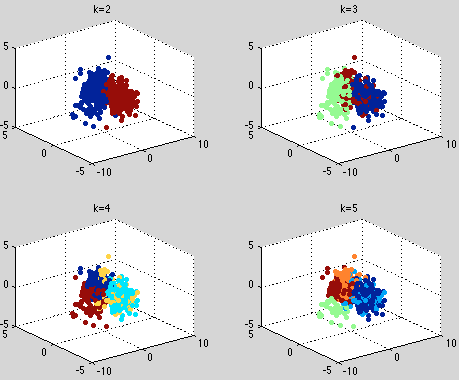
\includegraphics[width=0.55\textwidth]{img/Diabetes_2}
	\caption{k-means clustering for diabetes data using PCA}
	\label{fig:diabetes_2}
\end{figure}
\paragraph{}As it can be seen, the result of the classification doesn't seem to have changed a lot. That is because the three dimensions plotted in both cases are the three most relevant dimensions according to the PCA algorithm. Since the transformed data has removed the noise mostly by reducing the influence of the other dimensions of the plot, and the data was more evenly distributed among the other dimensions, the classification result is similar.\\

If the new inner cluster inertia values are taken into account once the PCA has cleared the data, it can be seen that the inertia is reduced a lot, even though the final clusters are almost the same:
\begin{table}[ht!]
	\centering
	\begin{tabular}{|c|c|c|c|}
		\hline
		\rowcolor[gray]{0.85} \textbf{K=2}&\textbf{K=3}&\textbf{K=4}&\textbf{K=5}\\\hline
		2713.89&1955.84&1610.03&1408.60\\\hline
	\end{tabular}
	\label{tab:diabetesPCA}
	\caption{Inertia of the clusters using the PCA}
\end{table}
\paragraph{}This implies that the noise has been cleared. By reducing the noise, the individuals are closer together, and the distance to the centroids is shorter.
% subsection data_set_pima_indians_diabetes_database (end)
\subsection{Data set: Vehicle silhouettes} % (fold)
\label{sub:data_set_vehicle_silhouettes}
\textbf{File:} vehicle.arff\\

This dataset corresponds to a study of the classification of cars into four different kinds () according o their silhouette. The data originally used for the classification is composed of 18 variables, which are:
\begin{enumerate}
	\item COMPACTNESS     (average perim)**2/area  
	\item CIRCULARITY     (average radius)**2/area
	\item DISTANCE CIRCULARITY    area/(av.distance from border)**2
	\item RADIUS RATIO    (max.rad-min.rad)/av.radius
	\item PR.AXIS ASPECT RATIO    (minor axis)/(major axis)
	\item MAX.LENGTH ASPECT RATIO (length perp. max length)/(max length)
	\item SCATTER RATIO   (inertia about minor axis)/(inertia about major axis)
	\item ELONGATEDNESS           area/(shrink width)**2
	\item PR.AXIS RECTANGULARITY  area/(pr.axis length*pr.axis width)
	\item MAX.LENGTH RECTANGULARITY area/(max.length*length perp. to this)
	\item SCALED VARIANCE ALONG MAJOR AXIS        (2nd order moment about minor axis)/area
	\item SCALED VARIANCE ALONG MINOR AXIS         (2nd order moment about major axis)/area
	\item SCALED RADIUS OF GYRATION       (mavar+mivar)/area
	\item SKEWNESS ABOUT MAJOR AXIS (3rd order moment about major axis)/sigma\_min**3
	\item SKEWNESS ABOUT MINOR AXIS (3rd order moment about minor axis)/sigma\_maj**3
	\item KURTOSIS ABOUT MINOR AXIS (4th order moment about major axis)/sigma\_min**4 
	\item KURTOSIS ABOUT MAJOR AXIS (4th order moment about minor axis)/sigma\_maj**4
	\item HOLLOWS RATIO   (area of hollows)/(area of bounding polygon)
\end{enumerate}
\paragraph{}The first step in the analysis of the data will be to try a classification of the individuals by using the K-Means classifer with different values of K. The plots~\ref{fig:Car_1} show the result of this classification.
\begin{figure}[ht!]
	\centering
	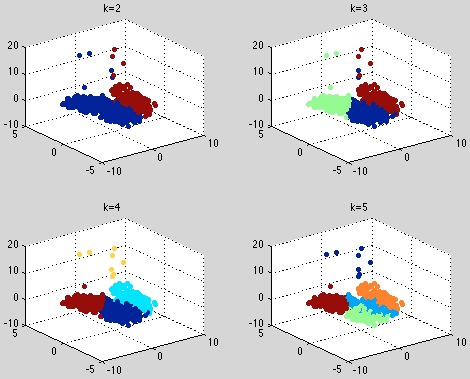
\includegraphics[width=0.55\textwidth]{img/Cars_1}
	\caption{k-means clustering for vehicle data without use PCA}
	\label{fig:Car_1}
\end{figure}
\paragraph{}As it can be seen in the plot, it seems the three first classifications are the best ones. For a value of K=2, two  very distinct groups of data are classified, and for K=3 the clustering seems to make an apparently unnatural division of the former first cluster into two distinct ones. In the case of K=4, although, it can be seen that a fourth cluster is made with those elements of the previous clusters that seemed to be outliers  in the previous clusters. To check if the increase of the clusters number is good, the inner cluster inertia can be checked:
\begin{table}[ht!]
	\centering
	\begin{tabular}{|c|c|c|c|}
		\hline
		\rowcolor[gray]{0.85} \textbf{K=2}&\textbf{K=3}&\textbf{K=4}&\textbf{K=5}\\\hline
		8958.65&7299.39&5973.53&5400.05\\\hline
	\end{tabular}
	\caption{Inertia of the clusters without use the PCA}
\end{table}
\paragraph{}As the number of clusters increases, as expected, the innertia decreases. But although the inertia doesn't decrease much when going from K=2 to K=3 (82.4\% of the inertia of K=2), it does when going from K=3 to K=4 (81\% of the inertia of K=3). It has to be taken into account that de pace of decrease in inertia is inversely proportional to the number of clusters. That is, as the number of clusters increases, the inertia decreases more slowly. For that reason, the 81\% of the inertia when going from K=3 to K=4 is much more significative than the same decrease when going from K=2 to K=3. It can be said that \underline{the best clustering in this case is for 4 clusters (K=4).}\\

An analysis by applying the PCA algorithm to the data set tells us that the most important components of the not discarded eigenvectors once applied an eigenvalue threshold of 1 are the 7th, 17th, 5th and 16th dimensions or attributes, in that order of relevance, which are:
\begin{itemize}
	\item 7.   Scatter ratio (inertia about minor axis)/(inertia about major axis)
	\item 17. Kurtosis about major axis (4th order moment about minor axis)/sigma\_maj**4
	\item 5.   Pr. Axis aspect ratio (minor axis)/(major axis)
	\item 16. Kurtosis about minor axis (4th order moment about major axis)/sigma\_min**4
\end{itemize}
\paragraph{}It's easy to see that attributes 7 and 5, which represent the distribution of force in the vehicle and the relative dimensions of the vehicle (width/length) are clearly influent when trying to describe a vehicle. Also, the Kurtosis attributes are important, since they describe the distribution of the forces along the two axis of the vehicle.\\

If the reduced dimensionality data obtained of the PCA by transforming the data set and then discarding the eigenvectors with a lower eigenvalue than 1 is used to classify the individuals, and then the individuals are plotted in the same coordinates space than before, the result is this one, figure~\ref{fig:Cars_2}.
\begin{figure}[ht!]
	\centering
	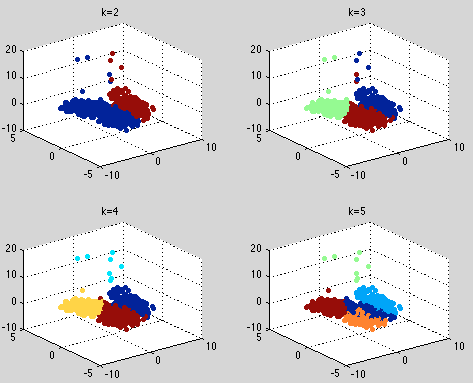
\includegraphics[width=0.55\textwidth]{img/Cars_2}
	\caption{k-means clustering for vehicle data using PCA}
	\label{fig:Cars_2}
\end{figure}

\paragraph{}It can be seen that the result is very similar to that of the first plot. This means that the reduction of dimensionality hasn't discarded any relevant dimensions. It can now be checked what has happened to the inner inertia of the clusters:
\begin{table}[ht!]
	\centering
	\begin{tabular}{|c|c|c|c|}
		\hline
		\rowcolor[gray]{0.85} \textbf{K=2}&\textbf{K=3}&\textbf{K=4}&\textbf{K=5}\\\hline
		6875.77&5234.29&3957.5551&3399.9879\\\hline
	\end{tabular}
	\caption{Inertia of the clusters using the PCA}
\end{table}
\paragraph{}It can be seen that now the inertia of K=4 is 75.6\% of that of k=3, meaning there is a greater reduction in inertia when increasing the number of clusters. This happens because now that the dimensionality is reduced, the individuals are closer together. It serves as a measure of the reduction of noise, but it can't be taken into account as a factor for determining a better separation between clusters, since the addition of a new cluster always has a greater impact in inertia if the space has a lower dimensionality.
% subsection data_set_vehicle_silhouettes (end)

\subsection{Data set: Wine recognition data} % (fold)
\label{sub:data_set_wine_recognition_data}
\textbf{File:} wine.arff\\

This is a data set used to classify wines coming from three different cultivars of the same region of italy. The goal would be to classify the different wines into their corresponding cultivars according to 13 different variables obtained from a chemical analysis of the wine.\\

In this case, there is no description to the 13 available attributes that are being analyzed, so they will be referred by their order in the data set with an integer value between 1 and 13.\\

The first step in the analysis of the data will be to try a classification of the individuals by using the K-Means classifier with different values of K. The plots \ref{fig:Wine_1}show the result of this classification.
\begin{figure}[ht!]
	\centering
	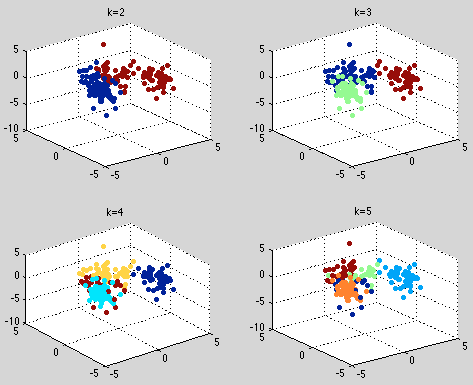
\includegraphics[width=0.55\textwidth]{img/Wines_1}
	\caption{k-means clustering for wines data without use PCA}
	\label{fig:Wine_1}
\end{figure}
\paragraph{}In this case, at plain sight, there appears to be a good clustering only in the case of K=3. For the case K=2  the red cluster is taking two groups of individuals which are clearly different, and for the case of K=4, there is a superposition between clusters, where the red and clear blue clusters are touching one with the other and there's no clear separation between them.\\

Even though, a good manner to check if it's really the case, is to check the reduction of the inner clusters inertia when the value of K increases.
\begin{table}[ht!]
	\centering
	\begin{tabular}{|c|c|c|c|}
		\hline
		\rowcolor[gray]{0.85} \textbf{K=2}&\textbf{K=3}&\textbf{K=4}&\textbf{K=5}\\\hline
		1649.44&1270.74&1168.77&1097.37\\\hline
	\end{tabular}
	\label{tab:cars}
	\caption{Inertia of the clusters without use the PCA}
\end{table}
\begin{itemize}
	\item Inertia of K=3 with respect to K=2: 77\%
	\item Inertia of K=4 with respect to K=3: 92\%
	\item Inertia of K=5 with respect to K=4: 94\%
\end{itemize}
\paragraph{}In this case, the inertia decreases when increasing the K value from 2 to 3, and has a very small decrease when further increasing the value of K.\\

For that reason, it can be said that \underline{the optimal K value is for K=3.}\\

An analysis by applying the PCA algorithm to the data set tells us that the most important components of the not discarded eigenvectors once applied an eigenvalue threshold of 1 are the 7th, 10th and 3rd dimensions or attributes, in that order of relevance.\\

If the reduced dimensionality data obtained of the PCA by transforming the data set and then discarding the eigenvectors with a lower eigenvalue than 1 is used to classify the individuals, and then the individuals are plotted in the same coordinates space than before, the result is this one, figure~\ref{fig:Wines_2}.
\begin{figure}[ht!]
	\centering
	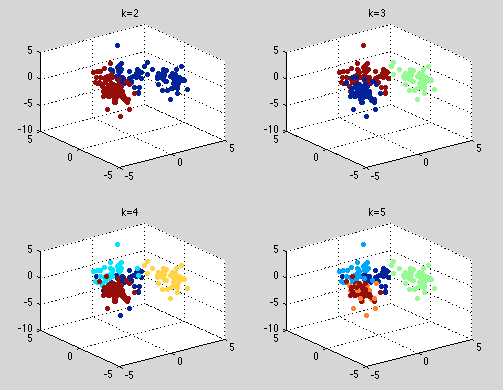
\includegraphics[width=0.55\textwidth]{img/Wines_2}
	\caption{k-means clustering for wines data using PCA}
	\label{fig:Wines_2}
\end{figure}
\paragraph{}The classification of the K-Means over the reduced dimensionality transformed data is, again, similar to that of the K-Means over the original data. As in the previous cases, this means that the reduced dimensionality has only discarded not relevant eigenvectors, and as such reduced the noise. As in the previous cases, this noise reduction can be seen by using the inner cluster inertia, which is lower than in the original data:
\begin{table}[ht!]
	\centering
	\begin{tabular}{|c|c|c|c|}
		\hline
		\rowcolor[gray]{0.85} \textbf{K=2}&\textbf{K=3}&\textbf{K=4}&\textbf{K=5}\\\hline
		881.18&510.11&427.05&368.32\\\hline
	\end{tabular}
	\label{tab:carsPCA}
	\caption{Inertia of the clusters using the PCA}
\end{table}
% subsection data_set_wine_recognition_data (end)
\subsection{Data set: Ionosphere} % (fold)
\label{sub:data_set_ionosphere}
\textbf{File:} inosphere.arff\\

This data set is a collection of information obtained from a ground array of antennas that analyzed data from the ionosphere and classified the individuals according to the existence of some structure in the ionosphere (good) and no structure at all (bad), which means the bombarded ions passed through the ionosphere and reached the ground.\\

The sampled data consists on 34 predictor attributes, all of them continuous and real.\\

The first step in the analysis of the data will be to try a classification of the individuals by using the K-Means classifier with different values of K. The following plots, figure~\ref{fig:Ionosphere_1} show the result of this classification.
\begin{figure}[ht!]
	\centering
	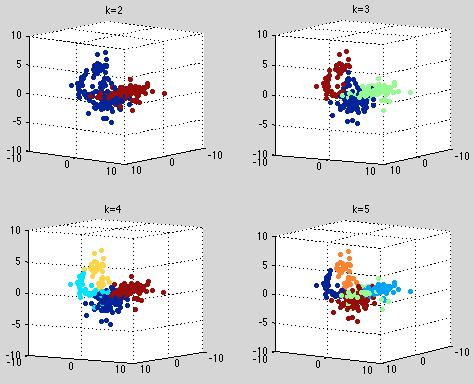
\includegraphics[width=0.55\textwidth]{img/Ionosphere_1}
	\caption{k-means clustering for ionosphere data without use PCA}
	\label{fig:Ionosphere_1}
\end{figure}
\paragraph{}Apparently, there seems to be a good separation between clusters for all values of K, specially for K=3 and K=4. This can be checked by comparing the differences inertia when K increases:
\begin{table}[ht!]
	\centering
	\begin{tabular}{|c|c|c|c|}
		\hline
		\rowcolor[gray]{0.85} \textbf{K=2}&\textbf{K=3}&\textbf{K=4}&\textbf{K=5}\\\hline
		9060.10&8238.18&7503.47&7101.62\\\hline
	\end{tabular}
	\caption{Inertia of the clusters without use the PCA}
\end{table}
\begin{itemize}
	\item Inertia of K=3 with respect to K=2: 91.0\%
	\item Inertia of K=4 with respect to K=3: 91.4\%
	\item Inertia of K=5 with respect to K=4: 94.6\%
\end{itemize}
\paragraph{}In this case, the small decrease in inertia in all cases show us that the apparent good classification of clusters with a value of K greater than 2 is just a result of the plot for the three most important dimensions, and thus, there must be some other important dimensions.\\

\underline{The best classification is for a value of K=2.}\\

An analysis by applying the PCA algorithm to the data set tells us that the most important components of the not discarded eigenvectors once applied an eigenvalue threshold of 1 are the 15th, 20th, 3rd, 34th, 1st, 8th and 24th dimensions or attributes, in that order of relevance. As proposed when analyzing the inertia with the K-Means, in this case there are many more important dimensions, a total of 7 compared to the 3 plotted.\\

If the reduced dimensionality data obtained of the PCA by transforming the data set and then discarding the eigenvectors with a lower eigenvalue than 1 is used to classify the individuals, and then the individuals are plotted in the same coordinates space than before, the result is this one, figure~\ref{fig:Ionosphere_2}
\begin{figure}[ht!]
	\centering
	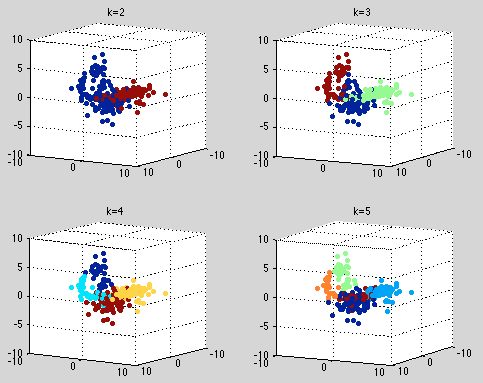
\includegraphics[width=0.55\textwidth]{img/Ionosphere_2}
	\caption{k-means clustering for ionosphere data using PCA}
	\label{fig:Ionosphere_2}
\end{figure}
\paragraph{}In that case, the K-Means classified the individuals in the same group as before in most of the cases, meaning that the noise has been discarded without affecting much the outcome. It can also be seen, though, that the red cluster for a K value of 5 is smaller, with some of its former individuals moved to the two blue clusters. That is, probably, because once the noise has been deleted, some elements have been moved closer together, and that fifth cluster was taking a range of noisy individuals to itself.\\
\newpage
If the new inertia for the K-Means algorithm is calculated, it can be seen that it is reduced, as the noise is lower and the elements are closer together:
\begin{table}[ht!]
	\centering
	\begin{tabular}{|c|c|c|c|}
		\hline
		\rowcolor[gray]{0.85} \textbf{K=2}&\textbf{K=3}&\textbf{K=4}&\textbf{K=5}\\\hline
		5702.83&4887.81&4174.16&3777.99\\\hline
	\end{tabular}
	\caption{Inertia of the clusters using the PCA}
\end{table}
% subsection data_set_ionosphere (end)
% section analysis_of_the_data_sets (end)

\end{document}
